\documentclass{article}

\usepackage{amsmath}
\usepackage{graphicx}
\usepackage{microtype}
\usepackage[margin=2.5cm]{geometry}
\usepackage{booktabs}
\usepackage{tabularx}
  \newcolumntype{C}{>{\centering\arraybackslash}X}
\usepackage{multirow}
  \newcommand{\minitab}[2][l]{\begin{tabular}{#1}#2\end{tabular}}
\usepackage{dcolumn}
  \newcolumntype{d}{D{.}{.}{3.1}}
\usepackage{setspace}
  \onehalfspacing
\usepackage[utopia]{mathdesign}

\renewcommand{\textfraction}{0.05}

\title{Water Filtration \\
       \large{ESE3401 Water \& Wastewater Engineering 1 Lab Report}}

\author{Mohanadas Harish Chandar \\
        U067314J}


\begin{document}
\maketitle

\section{Introduction}
An experiment was conducted to investigate the basic characteristics of 
different filter media used in the water filtration process. 
The composition of the filters investigated are given in 
Table~\ref{tab:filters_composition}. 
Each filter tube had a 172\,mm internal diameter, and contained approximately
80\,cm of filter media.

\begin{table}[htbp]
\centering
\begin{tabularx}{0.75\textwidth}{CCCCC} \toprule
 &  & \multicolumn{ 3}{c}{Weight (g)} \\ \cmidrule(lr){3-5}
 &  & Filter 1 & Filter 2 & Filter 3 \\ 
\multirow{-3}*{\minitab[c]{Sieve \\ Designation \\ Number}} & \multirow{-3}*{\minitab[c]{Screen \\ Opening \\ (mm)}} & (Fine) & (Coarse) & (Mixed) \\ \midrule
7 & 2.40 &  & 250 &  \\ 
14 & 1.20 &  & 1250 & 750 \\ 
25 & 0.76 & 500 & 2000 & 1500 \\ 
36 & 0.42 & 2000 & 500 & 250 \\ 
72 & 0.21 & 1000 &  &  \\ 
100 & 0.15 & 500 &  &  \\ 
Gravel &  & 15\,cm & 15\,cm & 15\,cm \\ 
Anthracite & 2.50 &  &  & 15\,cm \\ \bottomrule
\end{tabularx}
\caption{Composition of the filters investigated.}
\label{tab:filters_composition}
\end{table}

Each filter media was evaluated for its general hydraulic characteristics, 
its ability to remove turbidity, and its performance during a backwash run.
The most favourable filter media was then recommended for use in the treatment 
of raw water.



\section{Objectives}
For each filter media:
\begin{enumerate}
\item Find relationship between filtration rate and head loss
\item Investiage effect of time length of filter run
  \begin{enumerate}
  \item Find relationship between time length of filter run and head loss
  \item Investigate ability in removing turbidity at end of filter run
  \end{enumerate}
\end{enumerate}



\section{Procedure}
\subsection{Relationship between filtration rate and head loss}
\begin{enumerate}
\item Turbid water was prepared and fed into a constant head tank.
\item Water was supplied from the constant head tank into each filter at 
      various flow rates. Flowrates from 0.4\,L/min\nobreakdash--1.2\,L/min 
      were used in steps of 0.2\,L/min.
\item For each flow rate, the head loss through each filter media was recorded.
\end{enumerate}


\subsection{Effect of time length of filter run}
\begin{enumerate}
\item Turbid water was prepared and fed into a constant head tank.
\item The initial turbidity of the prepared turbid water was measured.
\item Water was supplied from the constant head tank into each filter at 
      0.6\,L/min.
\item Head loss through the each filter was measured at the start of each 
      filter run.
\item For Filters II and III, subsequent measurements were taken at 5\,min 
      intervals.
\item For Filter I, subsequent measurements were taken at 1\,min intervals 
      till the 10th minute. Thereafter, measurements were taken at 5\,min
      intervals.
\item The filter runs were terminated when additional head loss increased
      to 0.30\,m or after 30\,min of operation.
\item Turbidity of effluent was measured for each filter.
\end{enumerate}



\section{Results}
\subsection{Relationship between filtration rate and head loss}
See Appendix~\ref{app:tables_H_V} for tabular results for each filter. 
Figure~\ref{fig:H_V} shows the plot of head loss, $H$, versus filtration rate,
$V$.

\begin{figure}[htbp]
\centering
% GNUPLOT: LaTeX picture with Postscript
\begingroup
  \makeatletter
  \providecommand\color[2][]{%
    \GenericError{(gnuplot) \space\space\space\@spaces}{%
      Package color not loaded in conjunction with
      terminal option `colourtext'%
    }{See the gnuplot documentation for explanation.%
    }{Either use 'blacktext' in gnuplot or load the package
      color.sty in LaTeX.}%
    \renewcommand\color[2][]{}%
  }%
  \providecommand\includegraphics[2][]{%
    \GenericError{(gnuplot) \space\space\space\@spaces}{%
      Package graphicx or graphics not loaded%
    }{See the gnuplot documentation for explanation.%
    }{The gnuplot epslatex terminal needs graphicx.sty or graphics.sty.}%
    \renewcommand\includegraphics[2][]{}%
  }%
  \providecommand\rotatebox[2]{#2}%
  \@ifundefined{ifGPcolor}{%
    \newif\ifGPcolor
    \GPcolorfalse
  }{}%
  \@ifundefined{ifGPblacktext}{%
    \newif\ifGPblacktext
    \GPblacktexttrue
  }{}%
  % define a \g@addto@macro without @ in the name:
  \let\gplgaddtomacro\g@addto@macro
  % define empty templates for all commands taking text:
  \gdef\gplbacktext{}%
  \gdef\gplfronttext{}%
  \makeatother
  \ifGPblacktext
    % no textcolor at all
    \def\colorrgb#1{}%
    \def\colorgray#1{}%
  \else
    % gray or color?
    \ifGPcolor
      \def\colorrgb#1{\color[rgb]{#1}}%
      \def\colorgray#1{\color[gray]{#1}}%
      \expandafter\def\csname LTw\endcsname{\color{white}}%
      \expandafter\def\csname LTb\endcsname{\color{black}}%
      \expandafter\def\csname LTa\endcsname{\color{black}}%
      \expandafter\def\csname LT0\endcsname{\color[rgb]{1,0,0}}%
      \expandafter\def\csname LT1\endcsname{\color[rgb]{0,1,0}}%
      \expandafter\def\csname LT2\endcsname{\color[rgb]{0,0,1}}%
      \expandafter\def\csname LT3\endcsname{\color[rgb]{1,0,1}}%
      \expandafter\def\csname LT4\endcsname{\color[rgb]{0,1,1}}%
      \expandafter\def\csname LT5\endcsname{\color[rgb]{1,1,0}}%
      \expandafter\def\csname LT6\endcsname{\color[rgb]{0,0,0}}%
      \expandafter\def\csname LT7\endcsname{\color[rgb]{1,0.3,0}}%
      \expandafter\def\csname LT8\endcsname{\color[rgb]{0.5,0.5,0.5}}%
    \else
      % gray
      \def\colorrgb#1{\color{black}}%
      \def\colorgray#1{\color[gray]{#1}}%
      \expandafter\def\csname LTw\endcsname{\color{white}}%
      \expandafter\def\csname LTb\endcsname{\color{black}}%
      \expandafter\def\csname LTa\endcsname{\color{black}}%
      \expandafter\def\csname LT0\endcsname{\color{black}}%
      \expandafter\def\csname LT1\endcsname{\color{black}}%
      \expandafter\def\csname LT2\endcsname{\color{black}}%
      \expandafter\def\csname LT3\endcsname{\color{black}}%
      \expandafter\def\csname LT4\endcsname{\color{black}}%
      \expandafter\def\csname LT5\endcsname{\color{black}}%
      \expandafter\def\csname LT6\endcsname{\color{black}}%
      \expandafter\def\csname LT7\endcsname{\color{black}}%
      \expandafter\def\csname LT8\endcsname{\color{black}}%
    \fi
  \fi
  \setlength{\unitlength}{0.0500bp}%
  \begin{picture}(7200.00,5040.00)%
    \gplgaddtomacro\gplbacktext{%
      \csname LTb\endcsname%
      \put(902,660){\makebox(0,0)[r]{\strut{} 0.05}}%
      \put(902,2338){\makebox(0,0)[r]{\strut{} 0.2}}%
      \put(902,3447){\makebox(0,0)[r]{\strut{} 0.5}}%
      \put(902,1499){\makebox(0,0)[r]{\strut{} 0.1}}%
      \put(902,4285){\makebox(0,0)[r]{\strut{} 1}}%
      \put(1034,440){\makebox(0,0){\strut{} 0.5}}%
      \put(5624,440){\makebox(0,0){\strut{} 1.5}}%
      \put(6826,440){\makebox(0,0){\strut{} 2}}%
      \put(3930,440){\makebox(0,0){\strut{} 1}}%
      \put(264,2718){\rotatebox{90}{\makebox(0,0){\strut{}H (m)}}}%
      \put(3930,110){\makebox(0,0){\strut{}$V$ (m$^3$/m$^2$/hr)}}%
    }%
    \gplgaddtomacro\gplfronttext{%
      \csname LTb\endcsname%
      \put(5839,4603){\makebox(0,0)[r]{\strut{}Filter 1 (Fine): $H=0.518V^{0.701}$, R$^2$=0.99}}%
      \csname LTb\endcsname%
      \put(5839,4383){\makebox(0,0)[r]{\strut{}Filter 2 (Coarse): $H=0.092V^{0.450}$, R$^2$=0.95}}%
      \csname LTb\endcsname%
      \put(5839,4163){\makebox(0,0)[r]{\strut{}Filter 3 (Mixed): $H=0.077V^{0.498}$, R$^2$=0.99}}%
    }%
    \gplbacktext
    \put(0,0){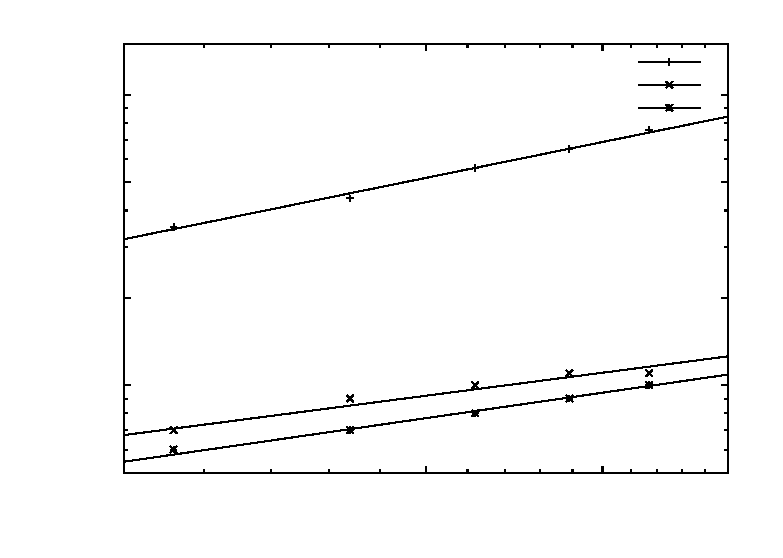
\includegraphics{H_V}}%
    \gplfronttext
  \end{picture}%
\endgroup

\caption{Log-log plot of head loss, $H$, versus filtration rate, $V$.}
\label{fig:H_V}
\end{figure}


\subsection{Effect of time length of filter run}
\subsubsection{Relationship between filtration rate and head loss}
See Appendix~\ref{app:tables_H_T} for tabular results for each filter. 
Figure~\ref{fig:H_T} shows the plot of head loss, $H$, versus 
time length of filter run, $T$.
\begin{figure}[htbp]
\centering
% GNUPLOT: LaTeX picture with Postscript
\begingroup
  \makeatletter
  \providecommand\color[2][]{%
    \GenericError{(gnuplot) \space\space\space\@spaces}{%
      Package color not loaded in conjunction with
      terminal option `colourtext'%
    }{See the gnuplot documentation for explanation.%
    }{Either use 'blacktext' in gnuplot or load the package
      color.sty in LaTeX.}%
    \renewcommand\color[2][]{}%
  }%
  \providecommand\includegraphics[2][]{%
    \GenericError{(gnuplot) \space\space\space\@spaces}{%
      Package graphicx or graphics not loaded%
    }{See the gnuplot documentation for explanation.%
    }{The gnuplot epslatex terminal needs graphicx.sty or graphics.sty.}%
    \renewcommand\includegraphics[2][]{}%
  }%
  \providecommand\rotatebox[2]{#2}%
  \@ifundefined{ifGPcolor}{%
    \newif\ifGPcolor
    \GPcolorfalse
  }{}%
  \@ifundefined{ifGPblacktext}{%
    \newif\ifGPblacktext
    \GPblacktexttrue
  }{}%
  % define a \g@addto@macro without @ in the name:
  \let\gplgaddtomacro\g@addto@macro
  % define empty templates for all commands taking text:
  \gdef\gplbacktext{}%
  \gdef\gplfronttext{}%
  \makeatother
  \ifGPblacktext
    % no textcolor at all
    \def\colorrgb#1{}%
    \def\colorgray#1{}%
  \else
    % gray or color?
    \ifGPcolor
      \def\colorrgb#1{\color[rgb]{#1}}%
      \def\colorgray#1{\color[gray]{#1}}%
      \expandafter\def\csname LTw\endcsname{\color{white}}%
      \expandafter\def\csname LTb\endcsname{\color{black}}%
      \expandafter\def\csname LTa\endcsname{\color{black}}%
      \expandafter\def\csname LT0\endcsname{\color[rgb]{1,0,0}}%
      \expandafter\def\csname LT1\endcsname{\color[rgb]{0,1,0}}%
      \expandafter\def\csname LT2\endcsname{\color[rgb]{0,0,1}}%
      \expandafter\def\csname LT3\endcsname{\color[rgb]{1,0,1}}%
      \expandafter\def\csname LT4\endcsname{\color[rgb]{0,1,1}}%
      \expandafter\def\csname LT5\endcsname{\color[rgb]{1,1,0}}%
      \expandafter\def\csname LT6\endcsname{\color[rgb]{0,0,0}}%
      \expandafter\def\csname LT7\endcsname{\color[rgb]{1,0.3,0}}%
      \expandafter\def\csname LT8\endcsname{\color[rgb]{0.5,0.5,0.5}}%
    \else
      % gray
      \def\colorrgb#1{\color{black}}%
      \def\colorgray#1{\color[gray]{#1}}%
      \expandafter\def\csname LTw\endcsname{\color{white}}%
      \expandafter\def\csname LTb\endcsname{\color{black}}%
      \expandafter\def\csname LTa\endcsname{\color{black}}%
      \expandafter\def\csname LT0\endcsname{\color{black}}%
      \expandafter\def\csname LT1\endcsname{\color{black}}%
      \expandafter\def\csname LT2\endcsname{\color{black}}%
      \expandafter\def\csname LT3\endcsname{\color{black}}%
      \expandafter\def\csname LT4\endcsname{\color{black}}%
      \expandafter\def\csname LT5\endcsname{\color{black}}%
      \expandafter\def\csname LT6\endcsname{\color{black}}%
      \expandafter\def\csname LT7\endcsname{\color{black}}%
      \expandafter\def\csname LT8\endcsname{\color{black}}%
    \fi
  \fi
  \setlength{\unitlength}{0.0500bp}%
  \begin{picture}(7200.00,5040.00)%
    \gplgaddtomacro\gplbacktext{%
      \csname LTb\endcsname%
      \put(902,660){\makebox(0,0)[r]{\strut{} 0.05}}%
      \put(902,2506){\makebox(0,0)[r]{\strut{} 0.2}}%
      \put(902,3726){\makebox(0,0)[r]{\strut{} 0.5}}%
      \put(902,1583){\makebox(0,0)[r]{\strut{} 0.1}}%
      \put(902,4649){\makebox(0,0)[r]{\strut{} 1}}%
      \put(1034,440){\makebox(0,0){\strut{} 0.01}}%
      \put(3930,440){\makebox(0,0){\strut{} 0.1}}%
      \put(6826,440){\makebox(0,0){\strut{} 1}}%
      \put(264,2718){\rotatebox{90}{\makebox(0,0){\strut{}H (m)}}}%
      \put(3930,110){\makebox(0,0){\strut{}$T$ (hr)}}%
    }%
    \gplgaddtomacro\gplfronttext{%
      \csname LTb\endcsname%
      \put(5839,4603){\makebox(0,0)[r]{\strut{}Filter 1 (Fine): Unable to suggest relation}}%
      \csname LTb\endcsname%
      \put(5839,4383){\makebox(0,0)[r]{\strut{}Filter 2 (Coarse): $H=0.109T^{0.087}$, R$^2$=0.74}}%
      \csname LTb\endcsname%
      \put(5839,4163){\makebox(0,0)[r]{\strut{}Filter 3 (Mixed): Unable to suggest relation}}%
    }%
    \gplbacktext
    \put(0,0){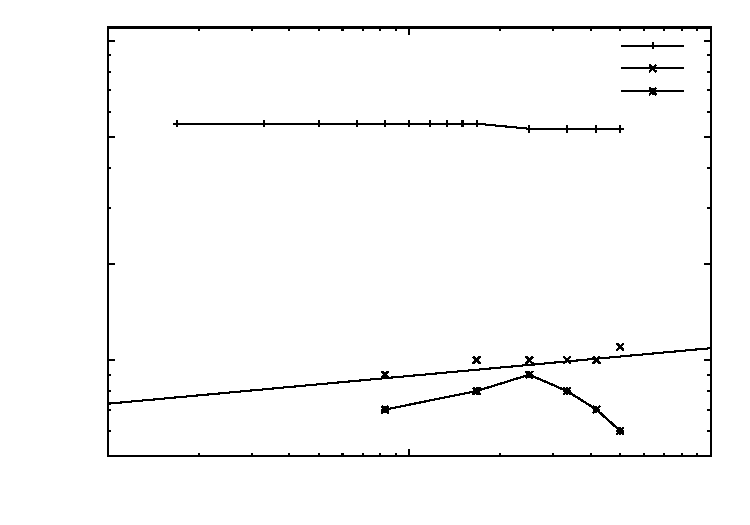
\includegraphics{H_T}}%
    \gplfronttext
  \end{picture}%
\endgroup

\caption{Log-log plot of head loss, $H$, versus time length of filter run, $T$.}
\label{fig:H_T}
\end{figure}

\subsubsection{Effect of time length of filter run}
Table~\ref{tab:turbidity} on page~\pageref{tab:turbidity} shows the turbidity
results obtained at end of each filter run.
\begin{table}[htbp]
\centering
\begin{tabular}{lccd} \toprule
 & \multicolumn{ 3}{c}{Turbidity (NTU)} \\ \cmidrule(lr){2-4}
 & Sample 1 & Sample 2 & \multicolumn{ 1}{c}{Average} \\ \midrule
Initial Turbidity &  &  & 796.5 \\ 
Filter 1 (Fine) Final & 50.7 & 49.8 & 50.3 \\ 
Filter 2 (Coarse) Final & 61.8 & 60.9 & 61.4 \\ 
Filter 3 (Mixed) Final & 55.6 & 55.8 & 55.7 \\ \bottomrule
\end{tabular}
\caption{Turbidity results at end of each filter run.}
\label{tab:turbidity}
\end{table}



\pagebreak
\section{Discussion}
\subsection{Relationship between filtration rate and head loss}
Figure~\ref{fig:H_V} and tables in Appendix~\ref{app:tables_H_V} summarize the 
fitration rate and head loss results.

Least squares regression was conducted on the data. 
Within the range of data, a $H=kV^n$ form of equation was optimal in relating 
head loss and filtration rate.
A linear relation was less successful for the coarse media filter.

After minor manual curve fitting, the following equations relating 
head loss and filtration are suggested:
\begin{center}
\begin{tabular}{rll}
Filter 1 (Fine): & $H=0.518V^{0.701}$ & R$^2$=0.99 \\
Filter 2 (Coarse): & $H=0.092V^{0.450}$ & R$^2$=0.95 \\
Filter 3 (Mixed): & $H=0.077V^{0.498}$ & R$^2$=0.99 \\
\end{tabular}
\end{center}

The fine media filter experienced the greatest head losses. 
It was also characterised by the largest exponent in the relationship between
filtration rate and head loss.
Thus, smaller pore sizes amplify the relationship between filtration rate and 
head loss.

\subsubsection{Relationship between finer media particles and head loss}
The mixed media filter had considerably more of its media retained on the 
largest sieve than the coarse media filter.
However, the head losses through both filters were fairly similar.
Furthermore, all filters included gravel, which appears to have little to no
comparative effect on head loss.

This strongly suggests that it is the finer particles in a media have the 
greatest effect on head loss.


\subsection{Effect of time length of filter run}
\subsubsection{Relationship between time length of filter run and head loss}
Figure~\ref{fig:H_T} and tables in Appendix~\ref{app:tables_H_T} summarize the 
length of filter run and head loss results.

Head loss was expected to increase over time, and the effect was expected to
be most pronounced for the fine media filter. 
However, no significant effect could be deduced from the data obtained.
A filtration run of 30\,min is thus insufficient to create a sufficient effect
on head loss.

A relationship between time length of filter run and head loss could only be 
suggested for the coarse media filter.
However, the suggested relation is only fairly representative due to the 
reasons given above.
\begin{center}
\begin{tabular}{rll}
Filter 2 (Coarse): & $H=0.109T^{0.087}$ & R$^2$=0.74 \\
\end{tabular}
\end{center}

\subsubsection{Ability in removing turbidity at end of filter run}
Table~\ref{tab:turbidity} summarizes the turbidity results at the end of the 
filter run.
The fine media filter had the best removal ability. Thus, smaller pore sizes 
improve removal ability.

The mixed media filter had a significantly better removal ability than the
coarse media filter. Furthermore, the pore sizes were comparable, or larger for the 
mixed media filter. 

Thus, anthracite has a significantly better turbidity removal ability than 
sand. This is probably due to the large surface area present in anthracite for
absorption.


\subsection{Backwash characteristics}
\subsubsection{Filter 1 (Fine)}
The fine media filter experienced a moderate rate of solids removal during backwash.
A low backwash pressure was sufficient to completely fluidize the media column.
However, there was considerable loss of filter media during the backwash.

\subsubsection{Filter 2 (Coarse)}
The coarse media filter experienced the slowest rate of solids removal during 
backwash. A high backwash pressure was required to fluidize the media column.

\subsubsection{Filter 3 (Mixed)}
The mixed media filter experienced the fastest rate of solids removal during 
backwash. The media column did not need to be fluidized completely for solids
removal. This is probably due to most of the solids being absorbed into the 
anthracite.



\section{Conclusion}
The relationship between filtration rate and head loss was found to be best
described in the form $H=kV^n$, where $H$ is head loss, $V$ is filtration rate
and $k$ and $n$ are constants. Linear relationships were less successful for 
the coarse media filter but could be used as a good approximation.
The fine media filter suffered significantly higher head loss than the coarse media and 
mixed media filters at all filtration rates.

A time length of 30\,min was found to be too short to suggest relationships
between time length of filter run and head loss.
The fine media and mixed media filters had better ability in removing turbidity at the end
of the filter run than the coarse media filter.

The mixed media filter had the most favourable backwash characteristics. 
It experienced the quickest solids removal, only required a low backwash 
pressure, and did not suffer from any noticeable loss of filter media.

Based on the the above experiemental findings, a mixed media filter is recommended 
for the treatment of raw water.



\clearpage
\appendix
\section{Additional tables}
\vfill
\subsection{Relationship between filtration rate and head loss}
\label{app:tables_H_V}
\begin{table}[htbp]
\centering
\begin{tabular}{ccccccc} \toprule
Flow rate, & Filtration rate, &  &  & Head loss, \\ 
$Q$ (L/min) & $V$ (10$^{-3}$\,m$^3$/m$^2$/hr) & $P_\text{top}$ (kPa) & $P_\text{bot}$ (kPa) & $H$ (m) \\ \midrule
0.4 & 0.56 & 14.9 & 19.3 & 0.35 \\ 
0.6 & 0.84 & 14.8 & 18.3 & 0.44 \\ 
0.8 & 1.12 & 14.7 & 17.1 & 0.56 \\ 
1.0 & 1.39 & 14.5 & 16.0 & 0.65 \\ 
1.2 & 1.67 & 14.3 & 14.7 & 0.76 \\ \bottomrule
\end{tabular}
\caption{Filtration rate and head loss results for Filter 1 (Fine)}
\label{tab:H_V_filter1}
\end{table}

\vfill
\begin{table}[htbp]
\centering
\begin{tabular}{ccccc} \toprule
Flow rate, & Filtration rate, &  &  & Head loss, \\ 
$Q$ (L/min) & $V$ (10$^{-3}$\,m$^3$/m$^2$/hr) & $P_\text{top}$ (kPa) & $P_\text{bot}$ (kPa) & $H$ (m) \\ \midrule
0.4 & 0.56 & 15.0 & 22.2 & 0.07 \\ 
0.6 & 0.84 & 14.9 & 21.9 & 0.09 \\ 
0.8 & 1.12 & 14.8 & 21.7 & 0.10 \\ 
1.0 & 1.39 & 14.7 & 21.5 & 0.11 \\ 
1.2 & 1.67 & 14.6 & 21.4 & 0.11 \\ \bottomrule
\end{tabular}
\caption{Filtration rate and head loss results for Filter 2 (Coarse)}
\label{tab:H_V_filter2}
\end{table}

\vfill
\begin{table}[htbp]
\centering
\begin{tabular}{ccccc} \toprule
Flow rate, & Filtration rate, &  &  & Head loss, \\ 
$Q$ (L/min) & $V$ (10$^{-3}$\,m$^3$/m$^2$/hr) & $P_\text{top}$ (kPa) & $P_\text{bot}$ (kPa) & $H$ (m) \\ \midrule
0.4 & 0.56 & 15.0 & 22.3 & 0.06 \\ 
0.6 & 0.84 & 14.9 & 22.1 & 0.07 \\ 
0.8 & 1.12 & 14.8 & 21.9 & 0.08 \\ 
1.0 & 1.39 & 14.7 & 21.7 & 0.09 \\ 
1.2 & 1.67 & 14.6 & 21.5 & 0.10 \\ \bottomrule
\end{tabular}
\caption{Filtration rate and head loss results for Filter 3 (Mixed)}
\label{tab:H_V_filter3}
\end{table}
\vfill


\clearpage
\subsection{Effect of time length of filter run}
\label{app:tables_H_T}
\begin{table}[htbp]
\centering
\begin{tabular}{ccccc} \toprule
Time, &  &  & Head loss, & Time, \\ 
(s) & $P_\text{top}$ (kPa) & $P_\text{bot}$ (kPa) & $H$ (m) & $T$ (h) \\ \midrule
0 & 14.7 & 17.2 & 0.55 & 0.000 \\ 
1 & 14.7 & 17.2 & 0.55 & 0.017 \\ 
2 & 14.7 & 17.2 & 0.55 & 0.033 \\ 
3 & 14.7 & 17.2 & 0.55 & 0.050 \\ 
4 & 14.7 & 17.2 & 0.55 & 0.067 \\ 
5 & 14.7 & 17.2 & 0.55 & 0.083 \\ 
6 & 14.7 & 17.2 & 0.55 & 0.100 \\ 
7 & 14.7 & 17.2 & 0.55 & 0.117 \\ 
8 & 14.6 & 17.1 & 0.55 & 0.133 \\ 
9 & 14.6 & 17.1 & 0.55 & 0.150 \\ 
10 & 14.6 & 17.1 & 0.55 & 0.167 \\ 
15 & 14.3 & 16.9 & 0.53 & 0.250 \\ 
20 & 14.1 & 16.7 & 0.53 & 0.333 \\ 
25 & 13.9 & 16.5 & 0.53 & 0.417 \\ 
30 & 13.7 & 16.3 & 0.53 & 0.500 \\ \bottomrule
\end{tabular}
\caption{Time length of filter run and head loss results for Filter 1 (fine).}
\label{tab:H_T_filter1}
\end{table}
\vfill

\begin{table}[htbp]
\centering
\begin{tabular}{ccccc} \toprule
Time, &  &  & Head loss, & Time, \\ 
(s) & $P_\text{top}$ (kPa) & $P_\text{bot}$ (kPa) & $H$ (m) & $T$ (h) \\ \midrule
0 & 14.9 & 21.8 & 0.10 & 0.000 \\ 
5 & 14.7 & 21.7 & 0.09 & 0.083 \\ 
10 & 14.6 & 21.5 & 0.10 & 0.167 \\ 
15 & 14.4 & 21.3 & 0.10 & 0.250 \\ 
20 & 14.2 & 21.1 & 0.10 & 0.333 \\ 
25 & 13.9 & 20.8 & 0.10 & 0.417 \\ 
30 & 13.7 & 20.5 & 0.11 & 0.500 \\ \bottomrule
\end{tabular}
\caption{Time length of filter run and head loss results for Filter 2 (coarse).}
\label{tab:H_T_filter2}
\end{table}
\vfill

\nopagebreak
\begin{table}[htbp]
\centering
\begin{tabular}{ccccc} \toprule
Time, &  &  & Head loss, & Time, \\ 
(s) & $P_\text{top}$ (kPa) & $P_\text{bot}$ (kPa) & $H$ (m) & $T$ (h) \\ \midrule
0 & 14.8 & 22.0 & 0.07 & 0.000 \\ 
5 & 14.8 & 22.0 & 0.07 & 0.083 \\ 
10 & 14.7 & 21.8 & 0.08 & 0.167 \\ 
15 & 14.5 & 21.5 & 0.09 & 0.250 \\ 
20 & 14.2 & 21.3 & 0.08 & 0.333 \\ 
25 & 14.0 & 21.2 & 0.07 & 0.417 \\ 
30 & 13.7 & 21.0 & 0.06 & 0.500 \\ \bottomrule
\end{tabular}
\caption{Time length of filter run and head loss results for Filter 3 (mixed).}
\label{tab:H_T_filter3}
\end{table}
\vfill

\end{document}
